\documentclass{beamer}
% Use DS9 global theme (includes pgfplots for visualization)
\usepackage{../../../shared/templates/ds9_theme}

% Title page configuration
\title[Vector Analysis and Projectile Motion]{PHYS11 CH:3.3-3.4}
\subtitle{Vector Addition (Analytical) and Projectile Motion}
\author[Mr. Gullo]{Mr. Gullo}
\date[Aug 2025]{August 28, 2025}

\begin{document}

\frame{\titlepage}

\begin{frame}
\frametitle{Learning Objectives}
\begin{itemize}
    \item Use the analytical method to add and subtract vectors by resolving them into components.
    \pause
    \item Determine the magnitude and direction of a resultant vector using the Pythagorean theorem and trigonometric identities.
    \pause
    \item Define and analyze projectile motion as two independent motions: constant velocity horizontally and constant acceleration vertically.
    \pause
    \item Solve projectile motion problems for quantities like position, velocity, maximum height, and range.
\end{itemize}
\end{frame}

\section{Vector Addition: Analytical Method}

\begin{frame}
\frametitle{Key Concepts: Vector Components}
\begin{itemize}
    \item The \alert{analytical method} of vector addition involves using trigonometric functions to resolve vectors into their components.
    \pause
    \item Any two-dimensional vector can be expressed as the sum of its \alert{horizontal (x)} and \alert{vertical (y)} components.
    \pause
    \item These components are perpendicular to each other and are independent.
\end{itemize}
\begin{block}{Component Equations}
    For a vector $\vec{A}$ with magnitude $A$ at an angle $\theta$ from the positive x-axis:
    \begin{itemize}
        \item Horizontal component: $A_x = A \cos \theta$
        \item Vertical component: $A_y = A \sin \theta$
    \end{itemize}
\end{block}
\end{frame}

\begin{frame}
\frametitle{Concept Visualization: Vector Components}
\begin{block}{Context}
    We can visualize a vector as the hypotenuse of a right-angled triangle. The legs of the triangle represent its horizontal ($A_x$) and vertical ($A_y$) components.
\end{block}
\end{frame}

\begin{frame}
\frametitle{Visualization: Resolving a Vector}
\centering
\begin{tikzpicture}[scale=1.5]
    % Draw axes
    \draw[->, ds9grey] (-0.2,0) -- (4.5,0) node[below] {$x$};
    \draw[->, ds9grey] (0,-0.2) -- (0,3.5) node[left] {$y$};

    % Draw vector A
    \draw[->, line width=2pt, ds9gold] (0,0) -- (4,3) node[midway, above, sloped] {$\vec{A}$};

    % Draw components
    \draw[->, line width=1.5pt, ds9blue] (0,0) -- (4,0) node[midway, below] {$A_x$};
    \draw[->, line width=1.5pt, ds9red] (4,0) -- (4,3) node[midway, right] {$A_y$};

    % Draw angle
    \draw[ds9grey, line width=1pt] (0.8,0) arc (0:36.87:0.8);
    \node[ds9grey] at (1.1,0.25) {$\theta$};
\end{tikzpicture}
\end{frame}

\begin{frame}
\frametitle{Steps for Analytical Vector Addition}
To add vectors $\vec{A}$ and $\vec{B}$ to find the resultant $\vec{R} = \vec{A} + \vec{B}$:

\begin{enumerate}
    \item \alert{Resolve} each vector into its x and y components.
    \begin{itemize}
        \item $A_x = A \cos \theta_A$, $A_y = A \sin \theta_A$
        \item $B_x = B \cos \theta_B$, $B_y = B \sin \theta_B$
    \end{itemize}
    \pause
    \item \alert{Sum} the components in each direction to find the components of the resultant, $\vec{R}$.
    \begin{itemize}
        \item $R_x = A_x + B_x$
        \item $R_y = A_y + B_y$
    \end{itemize}
    \pause
    \item \alert{Calculate} the magnitude and direction of $\vec{R}$ using the Pythagorean theorem and trigonometry.
    \begin{itemize}
        \item Magnitude: $R = \sqrt{R_x^2 + R_y^2}$
        \item Direction: $\theta = \tan^{-1}\left(\frac{R_y}{R_x}\right)$
    \end{itemize}
\end{enumerate}
\end{frame}

\begin{frame}
\frametitle{I Do: Finding a Resultant Displacement}
\begin{block}{Problem ( \#16)}
Suppose you walk 18.0 m straight west and then 25.0 m straight north. How far are you from your starting point, and what is the compass direction of a line connecting your starting point to your final position?
\end{block}
\end{frame}

\begin{frame}[fragile]
\frametitle{I Do: Solution}
\begin{columns}
\column{0.5\textwidth}
\begin{block}{G - Givens}
\begin{itemize}
    \item $\vec{d_1} = 18.0 \text{ m, West}$ \\ ($\vec{d}_{1x} = -18.0$ m, $\vec{d}_{1y} = 0$ m)
    \item $\vec{d_2} = 25.0 \text{ m, North}$ \\ ($\vec{d}_{2x} = 0$ m, $\vec{d}_{2y} = 25.0$ m)
\end{itemize}
\end{block}
\pause
\begin{block}{U - Unknown}
\begin{itemize}
    \item Resultant displacement $\vec{R}$
    \item Magnitude $R$ and direction $\theta$
\end{itemize}
\end{block}
\pause
\begin{block}{E - Equations}
\begin{itemize}
    \item $R_x = d_{1x} + d_{2x}$
    \item $R_y = d_{1y} + d_{2y}$
    \item $R = \sqrt{R_x^2 + R_y^2}$
    \item $\theta = \tan^{-1}\left(\frac{|R_y|}{|R_x|}\right)$
\end{itemize}
\end{block}
\column{0.5\textwidth}
\begin{block}{S - Substitute (Components)}
$R_x = -18.0 \text{ m} + 0 \text{ m} = -18.0 \text{ m}$
$R_y = 0 \text{ m} + 25.0 \text{ m} = 25.0 \text{ m}$
\end{block}
\pause
\begin{block}{S - Substitute (Magnitude)}
$R = \sqrt{(-18.0 \text{ m})^2 + (25.0 \text{ m})^2}$
\end{block}
\pause
\begin{block}{S - Solve (Magnitude)}
$R = \sqrt{324 \text{ m}^2 + 625 \text{ m}^2} = \sqrt{949 \text{ m}^2}$
$R = 30.8$ m
\end{block}
\pause
\begin{block}{S - Solve (Direction)}
$\theta_{ref} = \tan^{-1}\left(\frac{25.0}{18.0}\right) = 54.2^\circ$ N of W.
\vspace{0.5em}
For compass direction (W of N):
$\phi = 90^\circ - 54.2^\circ = 35.8^\circ$
\vspace{0.5em}
\alert{Answer: 30.8 m at 35.8$^\circ$ W of N}
\end{block}
\end{columns}
\end{frame}

\begin{frame}
\frametitle{We Do: Vector Components}
\begin{block}{Problem ( \#18)}
You drive 7.50 km in a straight line in a direction 15$^\circ$ east of north. Find the distances you would have to drive straight east and then straight north to arrive at the same point.
\end{block}
\pause
\begin{columns}
\column{0.5\textwidth}
\begin{block}{G - Givens}
\begin{itemize}
    \item $\vec{R} = 7.50$ km
    \item Direction: 15$^\circ$ E of N
\end{itemize}
\end{block}
\begin{block}{U - Unknown}
\begin{itemize}
    \item North component, $D_N = R_y$
    \item East component, $D_E = R_x$
\end{itemize}
\end{block}
\column{0.5\textwidth}
\begin{block}{E - Equations}
First, find the angle $\theta$ from the positive x-axis (East).
$15^\circ$ E of N is $90^\circ - 15^\circ = \alert{75^\circ}$.
\begin{itemize}
    \item $R_x = R \cos \theta$
    \item $R_y = R \sin \theta$
\end{itemize}
\end{block}
\pause
\begin{block}{S \& S - Your Turn!}
Substitute the values and solve for $D_E$ and $D_N$.
\end{block}
\end{columns}
\end{frame}


\begin{frame}
\frametitle{You Do: Adding Multiple Vectors}
\begin{block}{Problem ( \#24)}
Suppose a pilot flies 40.0 km in a direction 60$^\circ$ north of east and then flies 30.0 km in a direction 15$^\circ$ north of east. Find her total distance R from the starting point and the direction $\theta$ of the straight-line path to the final position.
\end{block}
\begin{center}
\alert{Use the analytical method and the GUESS framework to solve.}
\end{center}
\end{frame}

\section{Projectile Motion}

\begin{frame}
\begin{center}
{\Huge \textbf{Projectile Motion}}
\end{center}
\end{frame}

\begin{frame}
\frametitle{Key Concepts: Projectile Motion}
\begin{itemize}
    \item A \alert{projectile} is an object upon which the only force acting is gravity.
    \pause
    \item \alert{Projectile motion} is the motion of such an object.
    \pause
    \item The key to analyzing projectile motion is to treat the horizontal and vertical components of motion \alert{independently}.
    \pause
    \begin{columns}
    \column{0.5\textwidth}
    \begin{block}{Horizontal Motion}
        \begin{itemize}
            \item Velocity is \textbf{constant}.
            \item Acceleration is \textbf{zero} ($a_x = 0$).
        \end{itemize}
    \end{block}
    \column{0.5\textwidth}
    \begin{block}{Vertical Motion}
        \begin{itemize}
            \item Velocity \textbf{changes}.
            \item Acceleration is \textbf{constant} and downwards ($a_y = -g \approx -9.80$ m/s$^2$).
        \end{itemize}
    \end{block}
    \end{columns}
\end{itemize}
\end{frame}

\begin{frame}
\frametitle{Concept Visualization: Independence of Motion}
\begin{block}{Context}
To illustrate that vertical motion under gravity is independent of horizontal motion, consider two balls starting at the same height. One is dropped vertically, and the other is launched horizontally at the same instant.
\end{block}
\vspace{1em}
\begin{center}
Despite their different horizontal paths, they will both hit the ground at the same time.
\end{center}
\end{frame}

\begin{frame}
\frametitle{Visualization: The Dropped vs. Fired Ball}
\centering
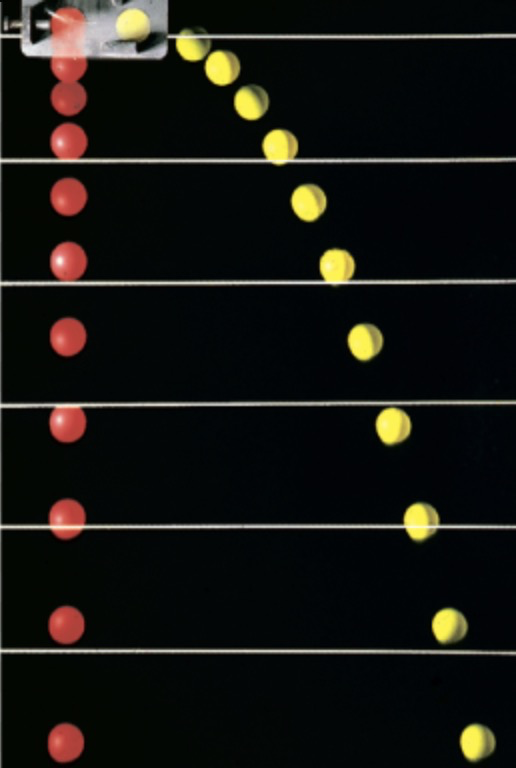
\includegraphics[width=0.8\linewidth]{phys12-projectile-motion-trajectory-analysis.png}
\end{frame}

\begin{frame}
\frametitle{Concept Visualization: Projectile Trajectory}
\begin{block}{Context}
The combination of constant horizontal velocity and constant vertical acceleration produces a curved path known as a \alert{trajectory}. If we ignore air resistance, this path is a perfect \alert{parabola}.
\end{block}
\end{frame}

\begin{frame}
\frametitle{Visualization: The Parabolic Path}
\begin{figure}
\begin{tikzpicture}
\begin{axis}[
    width=0.9\textwidth,
    height=0.6\textheight,
    axis lines=middle,
    xlabel={Horizontal Position (x) [m]},
    ylabel={Vertical Position (y) [m]},
    xmin=0, xmax=11,
    ymin=0, ymax=3,
    xtick={0,2,4,6,8,10},
    ytick={0,1,2,3},
    enlargelimits=true,
    xlabel style={anchor=north},
    ylabel style={anchor=east},
]
\addplot[domain=0:10, samples=50, ds9blue, line width=2pt] {x - 0.1*x^2};
\node[pin=135:{\small Max Height}] at (axis cs:5,2.5) {};
\end{axis}
\end{tikzpicture}
\end{figure}
\end{frame}

\begin{frame}[fragile]
\frametitle{Essential Equations: Projectile Motion}
\begin{columns}
\column{0.5\textwidth}
\begin{block}{Horizontal Motion ($a_x = 0$)}
\begin{itemize}
    \item $v_x = v_{0x}$ (constant)
    \item $x = x_0 + v_{0x}t$
\end{itemize}
\end{block}
\column{0.5\textwidth}
\begin{block}{Vertical Motion ($a_y = -g$)}
\begin{itemize}
    \item $v_y = v_{0y} - gt$
    \item $y = y_0 + v_{0y}t - \frac{1}{2}gt^2$
    \item $v_y^2 = v_{0y}^2 - 2g(y - y_0)$
\end{itemize}
\end{block}
\end{columns}
\pause
\begin{block}{Initial Velocity Components}
For an initial velocity $v_0$ at an angle $\theta_0$:
$v_{0x} = v_0 \cos \theta_0$ \quad and \quad $v_{0y} = v_0 \sin \theta_0$
\end{block}
\pause
\begin{block}{Special Case: Level Ground}
\begin{itemize}
    \item Range: $R = \frac{v_0^2 \sin(2\theta_0)}{g}$
    \item Max Height: $h = \frac{v_{0y}^2}{2g}$
\end{itemize}
\end{block}
\end{frame}

\begin{frame}
\frametitle{I Do: Horizontal Launch}
\begin{block}{Problem ( \#27)}
A ball is thrown horizontally from the top of a 60.0-m building and lands 100.0 m from the base of the building. Ignore air resistance.
\begin{enumerate}
    \item How long is the ball in the air?
    \item What was the initial horizontal velocity?
    \item What is the vertical component of the velocity just before it hits the ground?
\end{enumerate}
\end{block}
\end{frame}

\begin{frame}[fragile]
\frametitle{I Do: Solution}
\begin{block}{Givens}
\begin{itemize}
    \item Vertical: $y_0 = 60.0$ m, $y_f = 0$ m, $v_{0y} = 0$ m/s, $a_y = -9.80$ m/s$^2$
    \item Horizontal: $\Delta x = 100.0$ m, $a_x = 0$ m/s$^2$
\end{itemize}
\end{block}
\pause
\begin{block}{Part (a): Find time ($t$)}
\begin{itemize}
    \item \textbf{E:} Use vertical motion: $y_f = y_0 + v_{0y}t - \frac{1}{2}gt^2$
    \item \textbf{S:} $0 = 60.0 + (0)t - \frac{1}{2}(9.80)t^2$
    \item \textbf{S:} $-60.0 = -4.9t^2 \implies t = \sqrt{\frac{60.0}{4.9}} = \alert{3.50 \text{ s}}$
\end{itemize}
\end{block}
\pause
\begin{block}{Part (b): Find initial horizontal velocity ($v_{0x}$)}
\begin{itemize}
    \item \textbf{E:} Use horizontal motion: $\Delta x = v_{0x} t$
    \item \textbf{S:} $100.0 \text{ m} = v_{0x} (3.50 \text{ s})$
    \item \textbf{S:} $v_{0x} = \frac{100.0}{3.50} = \alert{28.6 \text{ m/s}}$
\end{itemize}
\end{block}
\end{frame}

\begin{frame}
\begin{block}{Part (c): Find final vertical velocity ($v_{fy}$)}
\begin{itemize}
    \item \textbf{E:} $v_{fy} = v_{0y} - gt$
    \item \textbf{S:} $v_{fy} = 0 - (9.80)(3.50)$
    \item \textbf{S:} $v_{fy} = \alert{-34.3 \text{ m/s}}$ (downward)
\end{itemize}
\end{block}
\end{frame}

\begin{frame}
\frametitle{We Do: Motorcycle Jump}
\begin{block}{Problem ( \#28)}
A daredevil attempts to jump his motorcycle over a line of buses by driving up a 32$^\circ$ ramp at a speed of 40.0 m/s. How many buses can he clear if the top of the takeoff ramp is at the same height as the bus tops and the buses are 20.0 m long?
\end{block}
\pause
\begin{block}{Givens \& Unknown}
\begin{itemize}
    \item \textbf{G:} $v_0 = 40.0$ m/s, $\theta_0 = 32^\circ$, Bus length = 20.0 m
    \item \textbf{U:} Number of buses cleared
\end{itemize}
\end{block}
\end{frame}

\begin{frame}
\begin{block}{Plan}
\begin{enumerate}
    \item This is a level-ground problem, so we can find the total horizontal distance (the Range). What equation should we use?
    \item \alert{Equation:} $R = \frac{v_0^2 \sin(2\theta_0)}{g}$
    \pause
    \item Let's substitute and solve for R.
    \item \alert{Substitute \& Solve:} $R = \frac{(40.0)^2 \sin(2 \times 32^\circ)}{9.80} = \frac{1600 \sin(64^\circ)}{9.80} = 146.7$ m
    \pause
    \item Now, how do we find the number of buses?
    \item \alert{Number of buses} = Total Range / Length of one bus
\end{enumerate}
\end{block}
\end{frame}

\begin{frame}
\frametitle{You Do: Archery Challenge}
\begin{block}{Problem ( \#29)}
An archer shoots an arrow at a 75.0 m distant target; the bull's-eye of the target is at same height as the release height of the arrow. At what angle must the arrow be released to hit the bull's-eye if its initial speed is 35.0 m/s?
\end{block}
\begin{center}
\alert{Hint: You will need to use the range equation and solve for the angle $\theta$.}
\end{center}
\end{frame}


\begin{frame}
\frametitle{Summary}
\begin{itemize}
    \item \textbf{Analytical Vector Addition}:
    \begin{itemize}
        \item Break vectors into x and y components using sine and cosine.
        \item Add components separately.
        \item Recombine using Pythagorean theorem and inverse tangent to find the resultant magnitude and direction.
    \end{itemize}
    \pause
    \item \textbf{Projectile Motion}:
    \begin{itemize}
        \item Motion in 2D under the influence of gravity alone.
        \item Horizontal motion has constant velocity ($a_x=0$).
        \item Vertical motion has constant acceleration ($a_y=-g$).
        \item The two components of motion are independent but share the same time, $t$.
        \item The resulting trajectory is a parabola.
    \end{itemize}
\end{itemize}
\end{frame}

\begin{frame}
\frametitle{Homework and Next Steps}

\begin{block}{Reading Assignment}
To prepare for our next topics and reinforce today's lesson, please read the following sections from Chapter 3:
\begin{itemize}
    \item \textbf{Sec 3.1}: Kinematics in Two Dimensions: An Introduction
    \item \textbf{Sec 3.2}: Vector Addition and Subtraction: Graphical Methods
    \item \textbf{Sec 3.5}: Addition of Velocities (focus on Relative Velocity)
\end{itemize}
\end{block}

\end{frame}

\end{document}